%% Copyright 2007 Ulf Lindgren
%
% This work may be distributed and/or modified under the conditions of the LaTeX
% Project Public License, either version 1.3 of this license or (at your option)
% any later version. The latest version of this license is in
%   http://www.latex-project.org/lppl.txt
% and version 1.3 or later is part of all distributions of LaTeX version
% 2005/12/01 or later.
%
% This work has the LPPL maintenance status `maintained'.
% 
% The Current Maintainer of this work is Ulf Lindgren.
%
% This work consists of all files listed in manifest.txt.
%
%% This statement added 2010/12/10 by Clea F. Rees following correspondence
%% between Ulf Lindgren and Karl Berry concerning licensing.

\documentclass{report}

 \setlength{\textheight}{23 cm}
 \setlength{\voffset}{-0.54cm}
 \setlength{\hoffset}{-0.54cm}
 \setlength{\oddsidemargin}{0.5 cm}
 \setlength{\evensidemargin}{0.5 cm}
 \setlength{\textwidth}{16 cm}
 \setlength{\marginparwidth}{2.5 cm}
 \setlength{\topmargin}{0.5 cm}
 \setlength{\headheight}{0.5 cm}
 \setlength{\headsep}{0.5 cm}

% \setlength{\voffset}{-5cm}
 \usepackage[T1]{fontenc}
 \usepackage[inputenc,babel]{translatex-fr}
  \usepackage{graphicx}
  \usepackage[Lenny]{fncychap}
  %\usepackage{ydrop}
  \usepackage{lettrine} % Pour remplacer ydrop qui ne donne pas les résultats attendus.

  \newcommand{\sk}{\vspace{0.2 cm}}
  \newcommand{\A}[1]{{$\backslash${\tt #1}}}
  \newcommand{\nsp}{\mbox{\hspace{-1 cm}}}
  \title{L'extension FncyChap\\V1.34}
  \author{Ulf A. Lindgren}
  \date{}
  

\begin{document}
  \maketitle
  \tableofcontents
  \chapter{Description de l'extension}
    \lettrine[findent=0.2em,nindent=0em,realheight=true]{L'}{extension} 
    \textsl{fncychap} a été écrite afin que des titres de niveau chapitre
    puissent être altérés rapidement et que je puisse apprendre plus sur
    \LaTeX{} et \TeX{}. Je ne sais pas si cette extension est écrite de façon
    adéquate. Aussi, si quelqu'un lit cette documentation et essaye 
    \textsl{fncychap}, je serais reconnaissant pour tout retour d'expérience. 
    Ceci m'aidera à monter compétence dans l'écriture de commandes. 
 
    Dans toute publication, il est essentiel de se rappeler que la cohérence
    joue un rôle important. Ainsi, avec cette extension, il est possible de
    modifier l'apparence de chaque chapitre séparément dans un document. Ceci
    n'est cependant pas souhaitable : n'oubliez ici pas la modestie et la 
    cohérence.

    \section{Chargement et utilisation classique}
    Cette extension est chargée en saisissant la ligne suivante en 
    préambule\sk\\    
    \nsp\fbox{\A{usepackage}[{\em style}]\{{\em fncychap}\}}\sk\\    
    Si l'option {\em style} est omise alors la définition par défaut des 
    chapitres est utilisée. À l'origine, il existait six styles de chapitres
    prédéfinis, à savoir {\em Sonny, Lenny, Glenn, Conny, Rejne} et 
    {\em Bjarne}. Ces noms correspondent à des prénoms suédois, à l'image sans 
    doute d'IKEA\footnote{Marque déposée d'Ingvar Kamprad Emtaryd Agunnaryd.}. 
    Chacun de ces styles dispose d'une configuration par défaut et, si elle
    est suffisante, il ne reste rien d'autre à faire.

    Dans la version actuelle de \textsl{fncychap}, deux styles additionnels
    ont été ajoutés. Le premier se nomme {\em PetersLenny}, d'après le nom de
    son auteur Peter Osborn. Ce style se base sur celui de {\em Lenny} : Peter
    a finement ajusté la taille des filets pour chacun des chapitres numérotés
    (jusqu'à 20) et chacune des annexes (jusqu'à Z). Le second style a été 
    défini par Jean-Marc François et il l'a nommé \textsl{Bjornstrup}.

    À l'origine, \textsl{fncychap} ne dépendait d'aucune autre extension. 
    Cependant, pour le style {\tt Lenny}, une fonte postscript est utilisée
    par défaut ; mais ceci peut être facilement changé. J'encourage 
    l'utilisation de cette fonte postscript par défaut car elle est 
    redimensionnable de façon très importante, ce qui rend {\em Lenny} 
    très agréable. Dans la version actuelle, si le style \textsl{Bjornstrup}
    de Jean-Marc est utilisé, l'extension \textsl{color} de la distribution de
    base sera chargée. 
    
  \chapter{Nouvelles commandes}
    \lettrine[findent=0.2em,nindent=0em,realheight=true]{E}{n} parallèle des 
    styles de chapitre, quelques commandes additionnelles sont mises à 
    disposition afin de créer ses titres de chapitre personnalisés.
    \tradini
  The commands
  will in the sequel be described. Each command is boxed and placed on
  a separate line. Lets begin the descriptions of the commands.\sk\\ 
  \nsp\fbox{\A{mghrulefill}\{{\em width}\}}\sk\\
  The above command is a more general version of the command
  \A{hrulefill} in the sense that the width of the ruler can be
  specified. This command is provided in order to decorate the chapter
  headers. The chapter heading are divided into two parts. The first
  part defines the so called \A{chapapp} and \A{thechapter} which
  holds information of the text ``Chapter'' and the current chapter number
  respectively. The second part is the chapter title provided by the
  user. From now one, the \A{chapapp} and \A{thechapter} will be
  referred to as chapter name and chapter number respectively. The
  user defined title is referred to as the chapter title.

  \section{Toward customization of the chapter head}
  \label{sec:TW}
    The chapter name, number and title can be changed easy, first lets
    introduce the following two commands\sk\\
    \nsp\fbox{\A{ChNameUpperCase}}\sk\\
    and\sk\\
    \nsp\fbox{\A{ChNameLowerCase}}\sk\\
    these commands will change the chapter name into either upper or
    lower case. One additional case command is provided for the
    chapter name, namely\sk\\
    \nsp\fbox{\A{ChNameAsIs}}\sk\\
    which result in the default case. Three similar commands for the
    chapter title are defined by the commands\sk\\
    \nsp\fbox{\A{ChTitleUpperCase}, \A{ChTitleLowerCase} and
      \A{ChNameAsIs}}\sk\\
    The rule width of the predefined chapter styles can be controlled
    by the command\sk\\
    \nsp\fbox{\A{ChRuleWidth}\{{\em width}\}}\sk\\
    just remember that the {\em width} must have a unit, for instance
    {\em pt, mm, etc}. The font related matters such as size, type and
    face can be sent using the commands\sk\\
    \nsp\fbox{\A{ChNameVar}\{{\em stuff}\}, \A{ChNumVar}\{{\em stuff}\} and
      \A{ChTitleVar}\{{\em stuff}\}}\sk\\
    related to the chapter name number and title respectively.
    The argument, {\em stuff}, to these functions can be for example
    \mbox{\A{ChNameVar}\{\A{huge}\A{rm}\A{centering}\}}.
    \enlargethispage{1cm}
  \chapter{An overview of the chapter styles}
    \lettrine[findent=0.2em,nindent=0em,realheight=true]{T}{he} chapter styles have default settings for all of the functions
    described in section~\ref{sec:TW}. However, it can be changed
    using the commands. Note that if \A{centering}, etc is used to
    format the text part of the chapter style then the result can be
    ugly. The chapter style {\em Bjarne} contains one additional
    command\sk\\
    \nsp\fbox{\A{TheAlphaChapter}}\sk\\
    This command will write the chapter number using the corresponding
    word. \A{TheAlphaChapter} have a capability of writing the words
    {\em ZERO} to {NINETYNINE}.
    

    In the following sections the pre-defined styles are shown along
    with the default settings. Both the \A{chapter} and \A{chapter*}
    are given.
    \section{The chapter Sonny}
    The following settings have been used as default parameters
    {\small\begin{verbatim}  
      \ChNameVar{\Large\sf}  \ChNumVar{\Huge}  \ChTitleVar{\Large\sf}
      \ChRuleWidth{0.5pt}    \ChNameUpperCase
    \end{verbatim}}    
    \begin{figure}[h]
      \begin{minipage}{7 cm}
        \label{fig:Sonnys}
        \centerline{\includegraphics[height=6cm]{Sonnys.eps}} 
        \caption{The stared chapter style sonny}
      \end{minipage}\hfill
      \begin{minipage}{7 cm}
        \label{fig:Sonny}
        \centerline{\includegraphics[height=6cm]{Sonny.eps}}
        \caption{The chapter style Sonny}
      \end{minipage}\hfill
    \end{figure}    
    
% \clearpage
    \section{The chapter Lenny}
    The following settings have been used as default parameters
    {\small\begin{verbatim}
      \ChNameVar{\fontsize{14}{16}\usefont{OT1}{phv}{m}{n}\selectfont}
      \ChNumVar{\fontsize{60}{62}\usefont{OT1}{ptm}{m}{n}\selectfont}
      \ChTitleVar{\Huge\bfseries\rm},  \ChRuleWidth{1pt}
    \end{verbatim}}
    \begin{figure}[h]
      \begin{minipage}{7 cm}
        \centerline{\includegraphics[height=6cm]{Lennys.eps}} 
        \caption{The stared chapter style Lenny}
      \end{minipage}\hfill
      \begin{minipage}{7 cm}
        \centerline{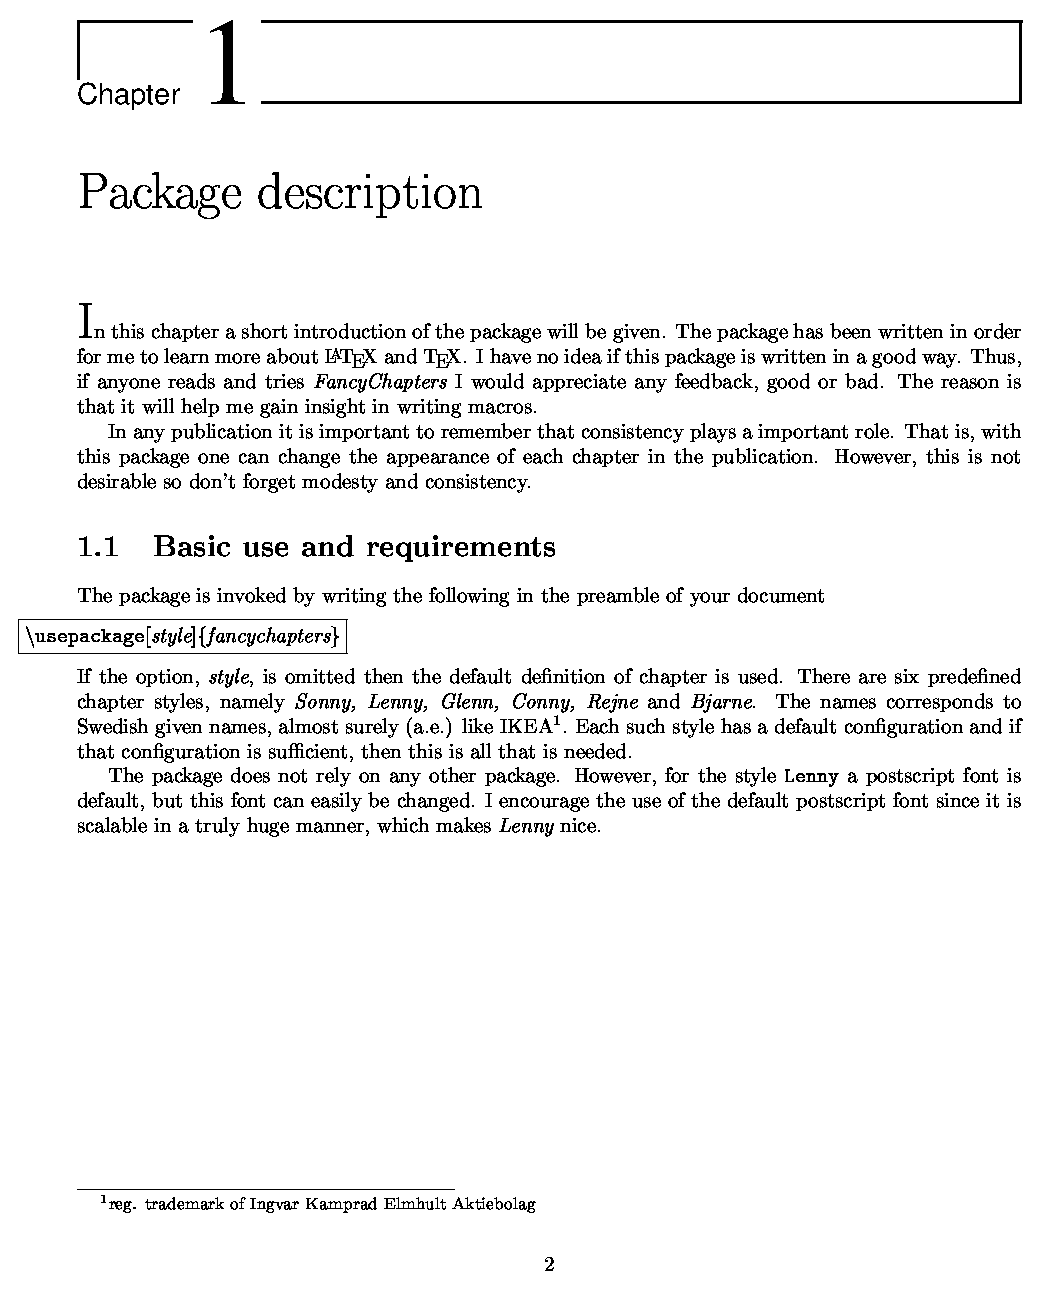
\includegraphics[height=6cm]{Lenny.eps}}
        \caption{The chapter style Lenny}
      \end{minipage}\hfill
    \end{figure}
\textbf{Note:} An alternative version of this chapter head exist
entitled \textsl{PetersLenny}.
%\enlargethispage{2cm}

    \section{The chapter Glenn}
    The following settings have been used as default parameters
    {\small\begin{verbatim}
      \ChNameVar{\bfseries\Large\sf},  \ChNumVar{\Huge},  \ChTitleVar{\bfseries\Large\rm}, 
      \ChRuleWidth{1pt},               \ChNameUpperCase,  \ChTitleUpperCase
    \end{verbatim}}
    \begin{figure}[h]
      \begin{minipage}{7 cm}
        \centerline{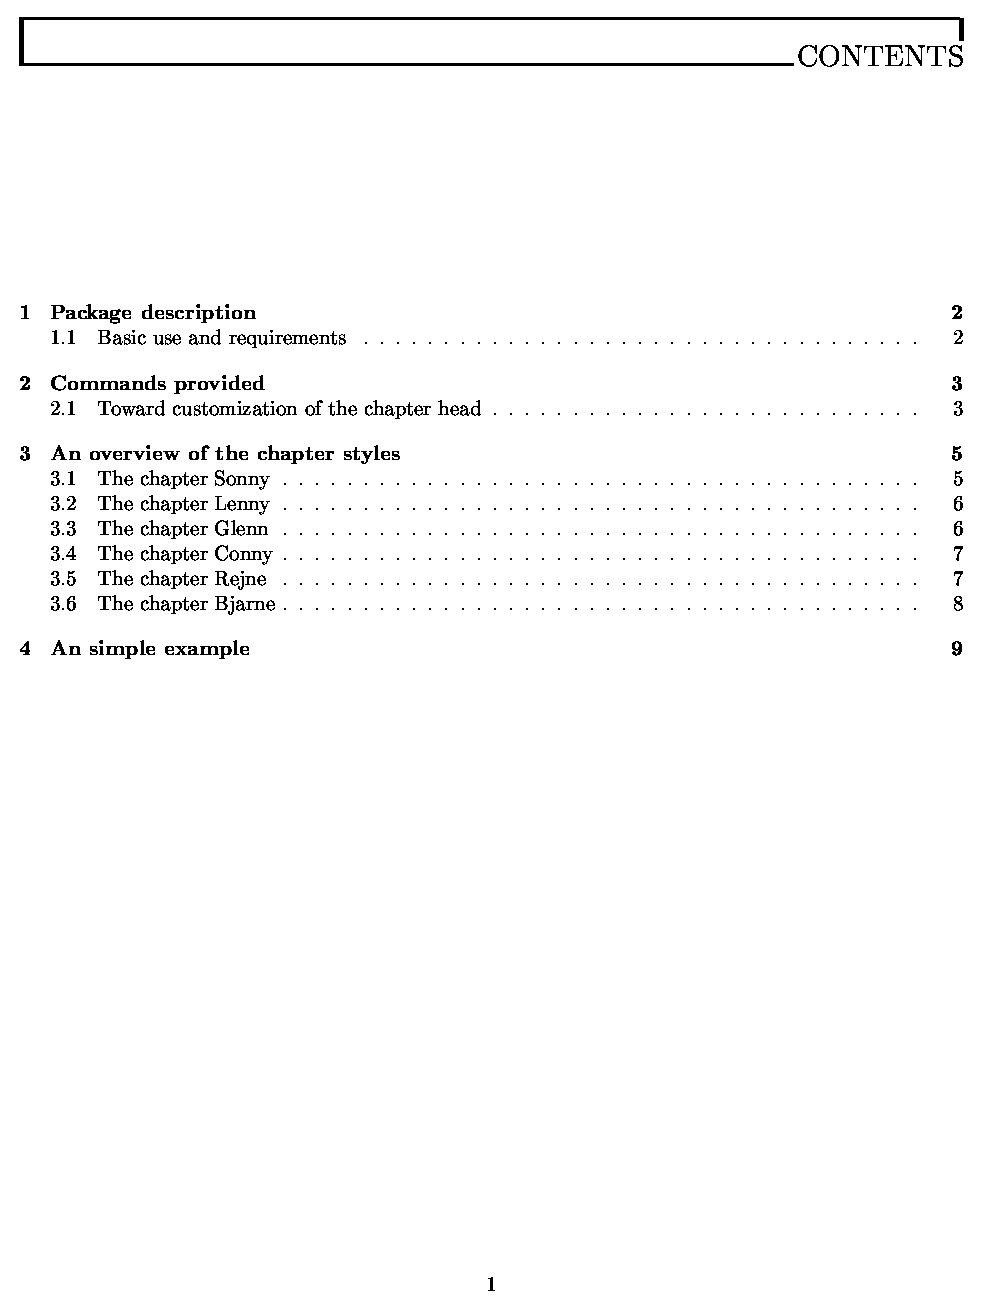
\includegraphics[height=6cm]{Glenns.eps}}
        \caption{The stared chapter style Glenn}
      \end{minipage}\hfill
      \begin{minipage}{7 cm}
        \centerline{\includegraphics[height=6cm]{Glenn.eps}}
        \caption{The chapter style Glenn}
      \end{minipage}\hfill
    \end{figure}

    \section{The chapter Conny}
    The following settings have been used as default parameters
    {\small\begin{verbatim}
       \ChNameUpperCase     \ChTitleUpperCase    \ChNameVar{\centering\Huge\rm\bfseries}
       \ChNumVar{\Huge}     \ChRuleWidth{2pt}    \ChTitleVar{\centering\Huge\rm}
    \end{verbatim}}
    \begin{figure}[h]
      \begin{minipage}{7 cm}
        \centerline{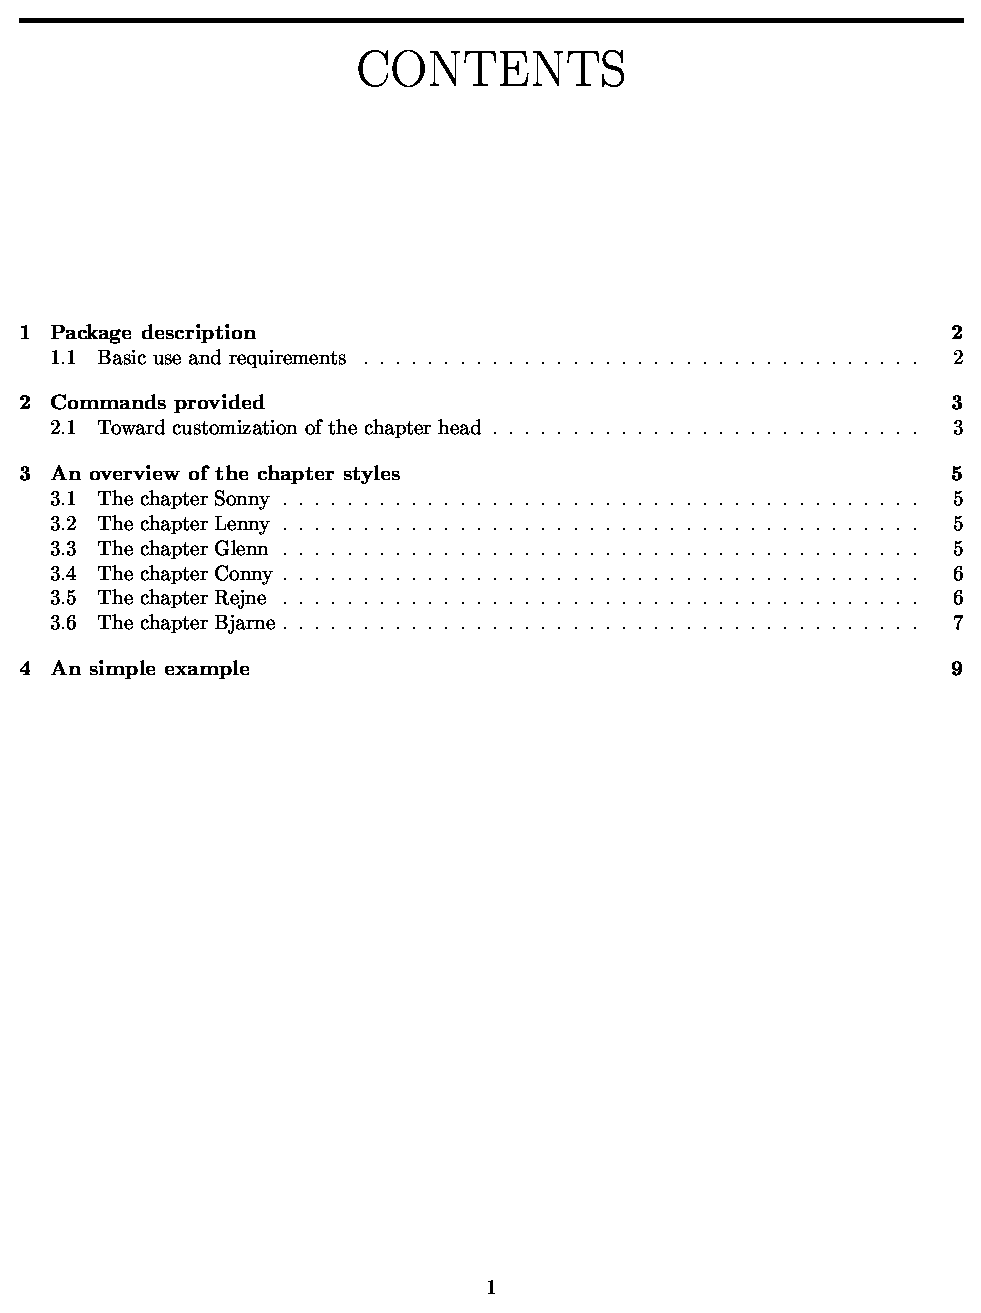
\includegraphics[height=6cm]{Connys.eps}}
        \caption{The stared chapter style Conny}
      \end{minipage}\hfill
      \begin{minipage}{7 cm}
        \centerline{\includegraphics[height=6cm]{Conny.eps}}
        \caption{The chapter style Conny}
      \end{minipage}\hfill
    \end{figure}

    \section{The chapter Rejne}
    The following settings have been used as default parameters\\
    {\small\begin{verbatim}  
      \ChNameVar{\centering\Huge\rm\bfseries}, \ChNumVar{\Huge},  \ChTitleVar{\centering\Huge\rm}
      \ChNameUpperCase,                        \ChTitleUpperCase, \ChRuleWidth{1pt}
   \end{verbatim}}
    \begin{figure}[h]
      \begin{minipage}{7 cm}
        \centerline{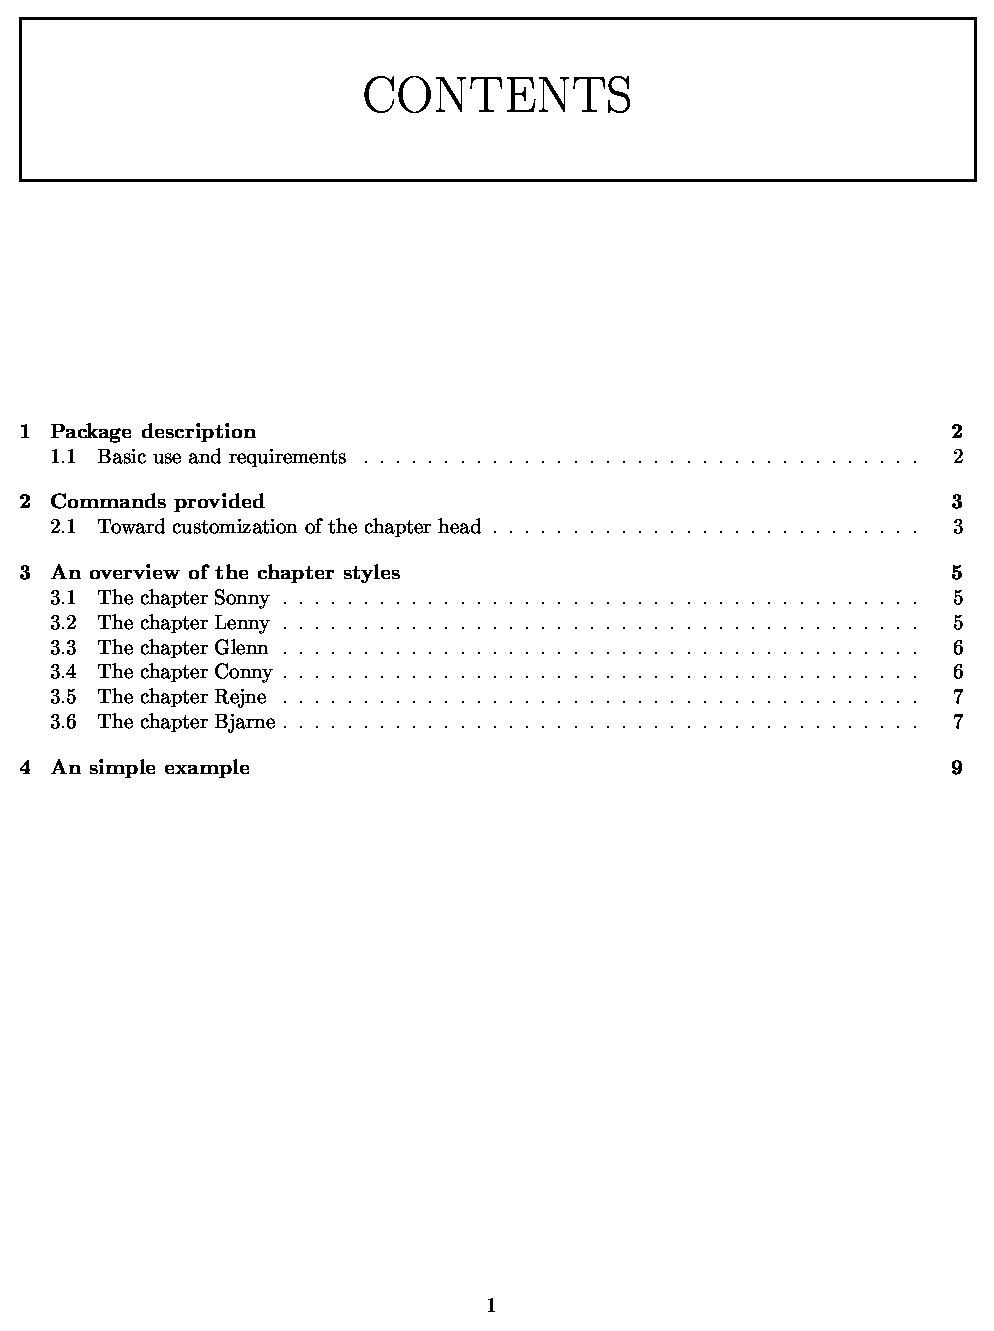
\includegraphics[height=6cm]{Rejnes.eps}}
        \caption{The stared chapter style Rejne}
      \end{minipage}\hfill
      \begin{minipage}{7 cm}
        \centerline{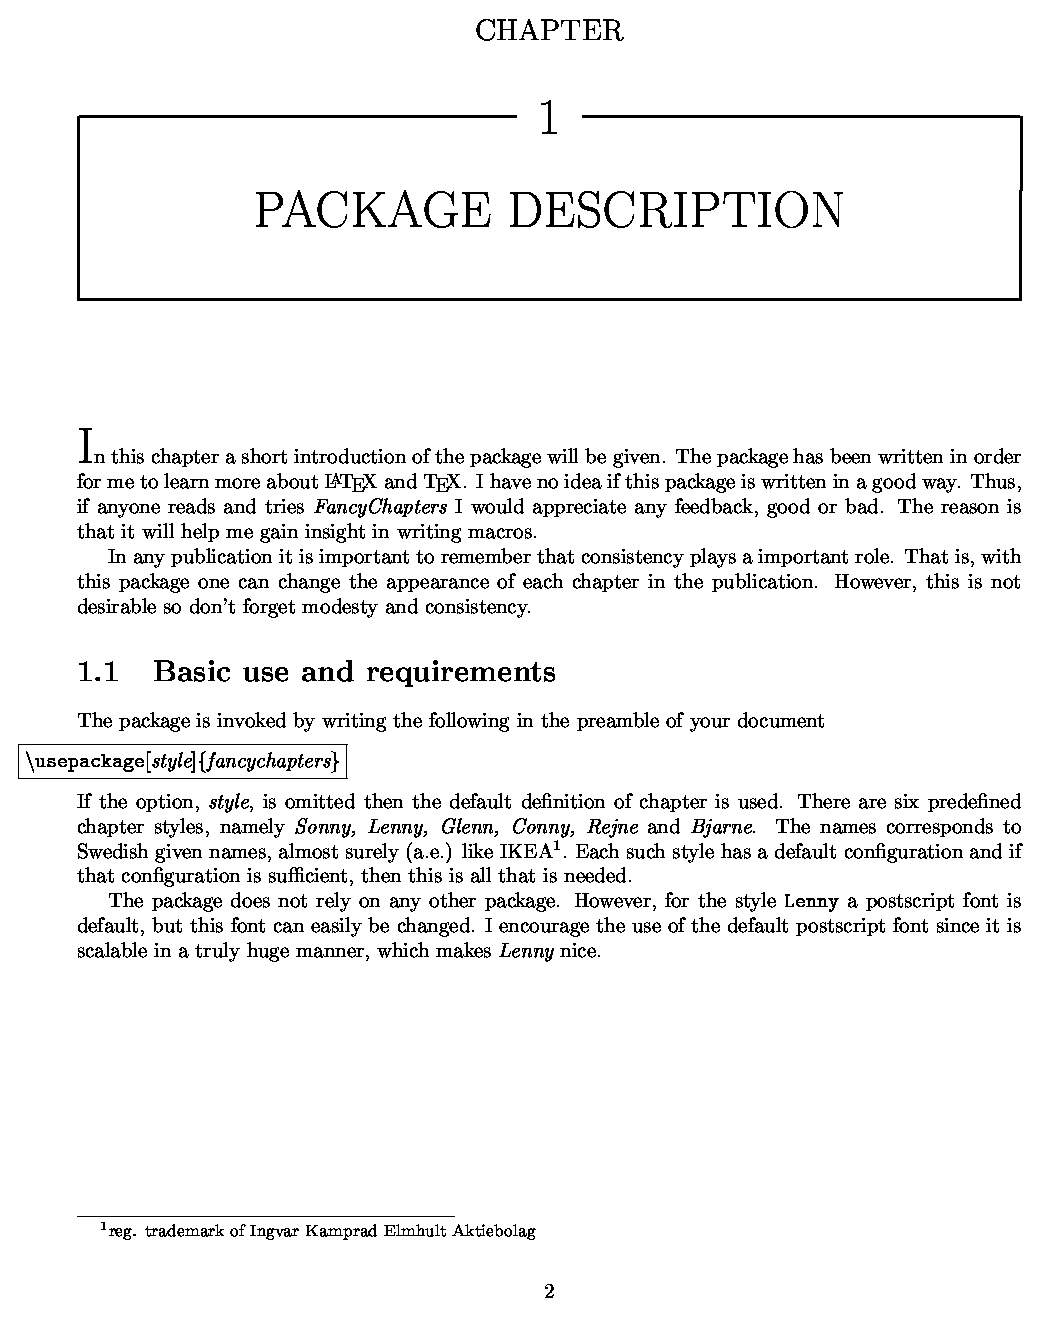
\includegraphics[height=6cm]{Rejne.eps}}
        \caption{The chapter style Rejne}
      \end{minipage}\hfill
    \end{figure}
    \section{The chapter Bjarne}
    The following settings have been used as default parameters\\
    {\small\begin{verbatim}
  \ChNameUpperCase   \ChNameVar{\raggedleft\normalsize\rm}   \ChRuleWidth{1pt}
  \ChTitleUpperCase  \ChNumVar{\raggedleft \bfseries\Large}  \ChTitleVar{\raggedleft \Large\rm}
     \end{verbatim}}
    \begin{figure}[h]
      \begin{minipage}{7 cm}
        \centerline{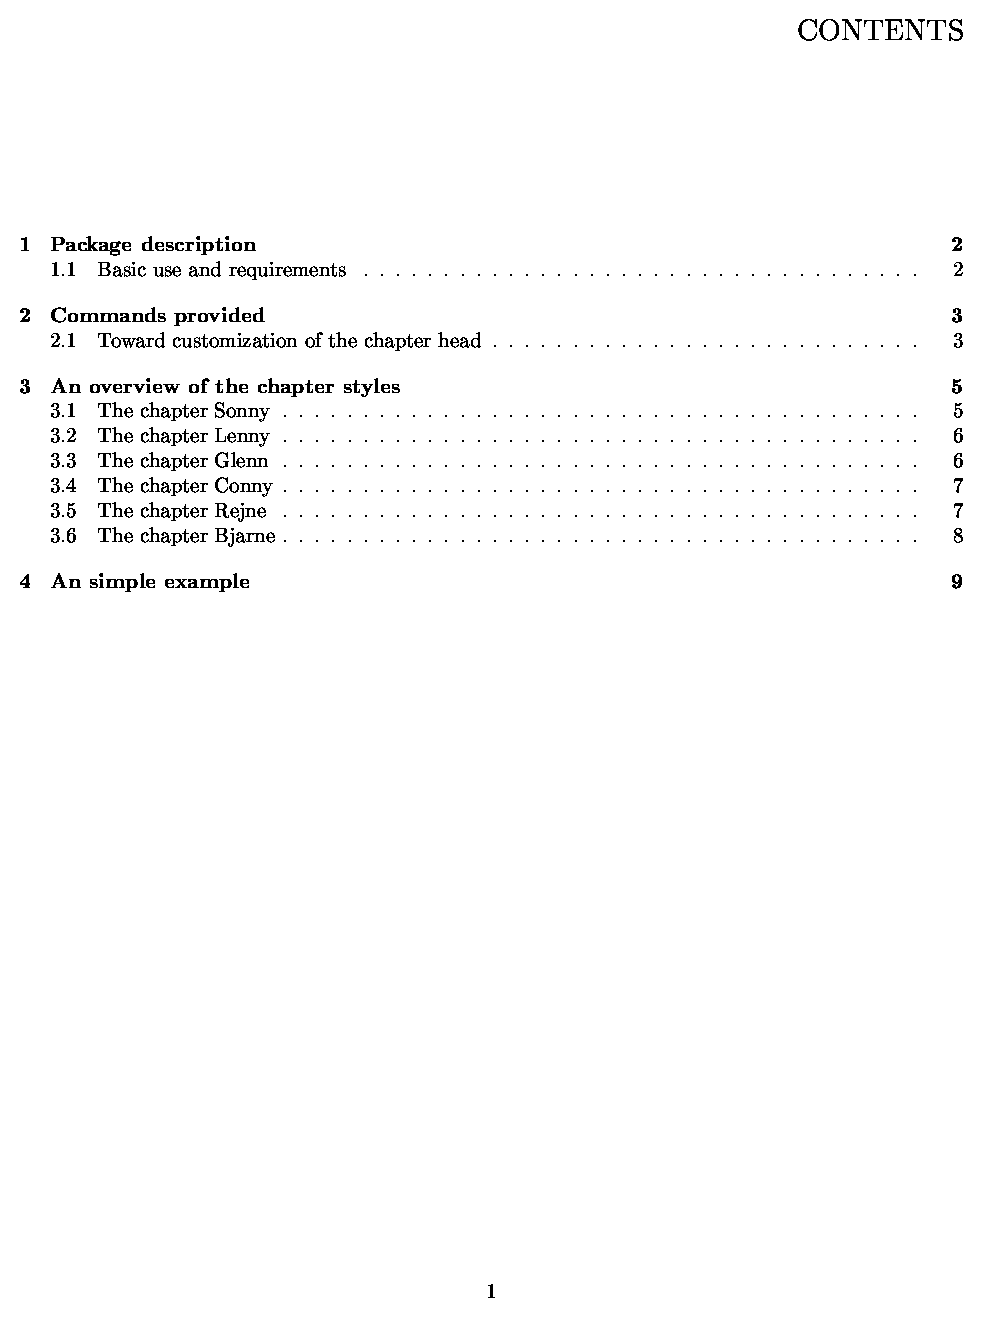
\includegraphics[height=6cm]{Bjarnes.eps}} 
        \caption{The stared chapter style Bjarne}
      \end{minipage}\hfill
      \begin{minipage}{7 cm}
        \centerline{\includegraphics[height=6cm]{Bjarne.eps}}
        \caption{The chapter style Bjarne}
      \end{minipage}\hfill
    \end{figure}

    \section{The chapter Bjornstrup}
    The following settings have been used as default parameters\\
    {\small\begin{verbatim}
  \ChNumVar{\fontsize{76}{80}\usefont{OT1}{pzc}{m}{n}\selectfont}
  \ChTitleVar{\raggedleft\Large\sffamily\bfseries}
  
     \end{verbatim}}
    \begin{figure}[h]
      \begin{minipage}{7 cm}
        \centerline{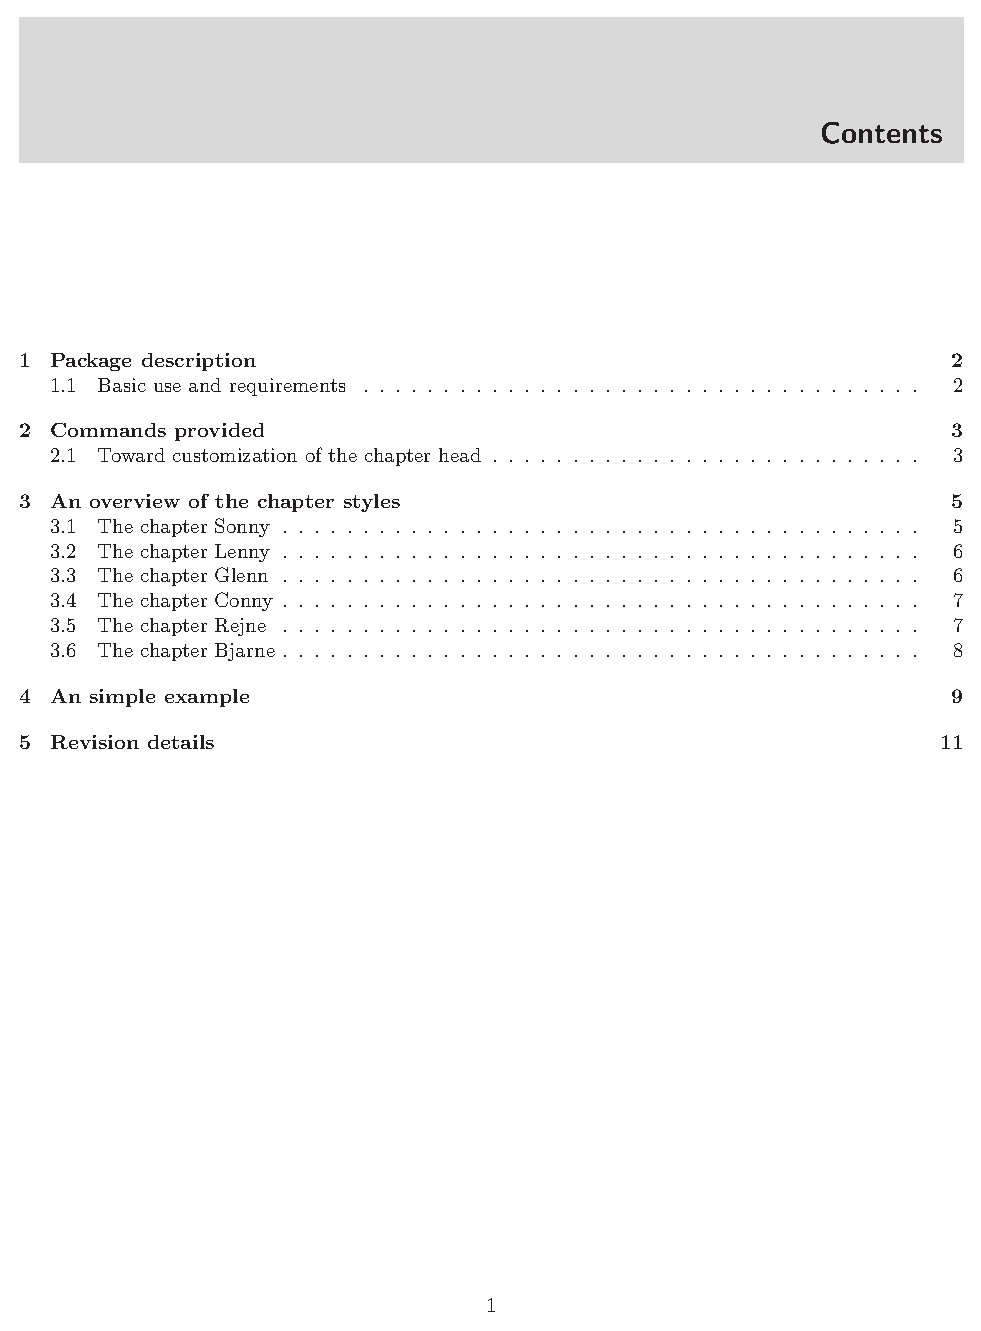
\includegraphics[height=6cm]{BjornstrupS.eps}} 
        \caption{The stared chapter style Bjornstrup}
      \end{minipage}\hfill
      \begin{minipage}{7 cm}
        \centerline{\includegraphics[height=6cm]{Bjornstrup.eps}}
        \caption{The chapter style Bjornstrup}
      \end{minipage}\hfill
    \end{figure}
\textbf{Note:} It appears as if the rendering in YAP (dvi previewer in
MikTeX) differs from dvips in that the gray box become
foreground. Thus, the chapter number is partly hidden. 
\enlargethispage{2cm}
  \chapter{A simple example}
    \lettrine[findent=0.2em,nindent=0em,realheight=true]{I}{f}
    the pre defined styles does not fulfill your needs then you can
    modify the formating routines. The formatting is controlled by
    three commands. One might as well redefine the original
    chapter definitions using the \A{secdef} and \A{renewcommand}, see
    The \LaTeX{} companion. However, at the time of creating this
    package I decided that this was easier. The command\sk\\
    \nsp\fbox{\A{DOCH}}\sk\\
    formats the chapter name and number. The commands\sk\\
    \nsp\fbox{\A{DOTI}\{{\#1}\}}\sk\\
    and\sk\\
    \nsp\fbox{\A{DOTIS}\{{\#1}\}}\sk\\
    formats the chapter title for \A{chapter} and \A{chapter*} respectively.
    In order to modify these you will have to use the preamble along
    with the commands \A{makeatletter} and \A{makeatother}. The in
    addition some predefined parameters can be used. The predefined
    length variables are\sk\\
    \nsp\fbox{\A{mylen}, \A{myhi}, \A{px}, \A{py}, \A{pxx}, \A{pyy}
      and \A{RW}}\sk\\
    note that \A{RW} is special, since it is set by \A{ChRuleWidth}.
    The formatting controlled by \A{ChNameVar}, \A{ChNumVar} and
    \A{ChTitleVar} store their values in \A{CNV}, \A{CNoV} and \A{CTV}
    respectively. Finally, The functions \A{FmN}\{ \} and \A{FmTi}\{
    \} acts accordingly to \A{Ch***AsIs}, \A{Ch***UpperCase} and
    \A{Ch***LowerCase}. Note that the stars indicate appropriate
    substitution of text, see section~\ref{sec:TW}.

    To illustrate this lets define a new chapter style in which the
    Chapter name and number in a \A{fbox} and the chapter title
    centered. The \A{fboxrule} is linked to the predefined length
    \A{RW} so that it can be controlled by the command
    \A{ChRuleWidth}. Try this example at a computer near you.
    \begin{verbatim}
       \makeatletter
         \ChNameVar{\Large\rm}    % sets the style for name
         \ChNumVar{\Huge}         % sets the style for digit
         \ChTitleVar{\Large\rm\centering}   % sets the style for title
         \ChRuleWidth{4pt}        % Set RW=4pt
         \ChNameUpperCase         % Make name uppercase
         \renewcommand{\DOCH}{%
           \setlength{\fboxrule}{\RW} % Let fbox lines be controlled by
                                      % \ChRuleWidth

           \fbox{\CNV\FmN{\@chapapp}\space \CNoV\thechapter}\par\nobreak
           \vskip 40\p@}

         \renewcommand{\DOTI}[1]{%
           \CTV\FmTi{#1}\par\nobreak
           \vskip 40\p@}
         \renewcommand{\DOTIS}[1]{%
           \CTV\FmTi{#1}\par\nobreak
           \vskip 40\p@}
       \makeatother
    \end{verbatim}
    That is all there is to it. Note that the commands \A{DOTI} and
    \A{DOTIS} can be redefined anywhere in the document, but that is
    not a good idea. Suppose that you want to use the
    \A{TheAlphaChapter}. This can be done by initially chose the style
    {\em Bjarne}\/ and then redefine \A{DOCH}, \A{DOTI} and \A{DOTIS}.
    \chapter{Revision details}

     \lettrine[findent=0.2em,nindent=0em,realheight=true]{T}{his} is version 1.34, some minor problems have been
     addressed and two new predefined chapter heads have been
     incorporated. The upper case and lower case handling have been
     corrected. A bad behavior in changes between \verb+\frontmatter+,
     \verb+\mainmatter+ and  \verb+\backmatter+, have been fixed.   

     In version 1.33 Rejne definition streched text caused ugly gaps
     in the vrule aligned with the title text. A compatibility problem
     with the KOMA class 'scrbook.cls' the remedy is a redefinition of
     '\@schapter' in line with that used in KOMA. This might not be
     good since it differs from the base definition. A spell error was
     corrected.
 
      In version 1.3, a problem with appendices in the Bjarne style was
      corrected. Wrong behavior, for the commands
      \verb+\frontmatter+, \verb+\mainmatter+ and  \verb+\backmatter+
      was dealt with. 

      In the release 1.11 of the current package. A bug
      fix of the Lenny option was included. The problem, reported
      by Diab Jerius, occurred (underfull vbox) when the option Lenny
      was used in conjunction with \A{section}-command such that the
      section is typeset at the next page. This caused one line to be
      misplaced. The remedy was to box the chapter title.

      In the release (1.1) of the current package. A
      modification was made such that it will work with the book
      class. The problem occurred when the fncychap styles Conny,
      Rejne, Bjarne or Glenn were used in conjunction with the
      \LaTeX{} command \A{tabelofcontents}. The exact reason for the
      error is not yet found. The problem was reported by Olivier Guibe.

      In the prior release there were no major improvements of the
      package. However, the package name was changed in order to
      conform with the (DOS) requirement of eight characters. I also
      received some feedback, informing me that the \LaTeX{} base have
      to be post 1994/12/01.  This information has been included in
      the package such that if an old base is used a warning will be
      written into the {\tt
        log}.\\
      Release history:
      \begin{description}
        \item[Release 1] 1996/12/13 FancyChapters 1.0b
        \item[Release 2] 1997/01/08 FncyChap 1.0 (Name change, base
          date option)
        \item[Release 3] 1997/01/22 FncyChap 1.1 (Bug fix)
        \item[Release 4] 1997/04/06 FncyChap 1.11 (Bug fix)
        \item[Release 5] 2004/09/20 FncyChap 1.3 (Bug fix)
        \item[Release 6] 2005/08/09 FncyChap 1.33 (Bug fix)
        \item[Release 7] 2007/07/31 FncyChap 1.34 (Bug fix)
      \end{description}

\end{document}
%%% Local Variables: 
%%% mode: latex
%%% TeX-master: t
%%% End: 
